\documentclass[pdflatex,sn-mathphys-num]{sn-jnl}

% === Basic Encoding and Language ===
\usepackage[T1,T2A]{fontenc}
\usepackage{cmap}
\usepackage[utf8]{inputenc}
\usepackage[english]{babel}

% === Math and Structure ===
\usepackage{amsmath, amssymb, amsthm}
\usepackage{tikz}
\usetikzlibrary{shapes.geometric,arrows.meta}
\usetikzlibrary{positioning}
\usepackage{xcolor}
\usepackage{booktabs}
\usepackage{tabularx}
\usepackage{ragged2e}
\usepackage{microtype}
\usepackage{hyperref}
\usepackage{textcomp}
\usepackage{float}
\usepackage{tcolorbox}
\usepackage{graphicx}
\DeclareGraphicsExtensions{.png,.pdf,.jpg}
\graphicspath{{./}}  % Specifies the current folder

% === Code and Formatting ===
\usepackage{fvextra}

% === Global Settings ===
\AtBeginDocument{\let\latexlabel\label}

% === Environment for Prompts Definition ===
\DefineVerbatimEnvironment{CodeBlock}{Verbatim}{
  breaklines=true,          % Line breaks allowed visually
  breaksymbolleft={},       % No left break symbol
  breaksymbolright={},      % No right break symbol
  fontsize=\small,          % Font size
  frame=single,             % Frame around the block
  commandchars=\\\{\},      % Allows \textbf{} etc.
  samepage=true             % Do not break the block across pages
}

% === CodeBlock Page Numbering Control ===
\usepackage{etoolbox}
\usepackage{afterpage}

\newif\ifinprompt
\inpromptfalse

% --- CodeBlock start ---
\AtBeginEnvironment{CodeBlock}{%
  \thispagestyle{empty}% Hide on the block's starting page
  \pagestyle{empty}% Hide on all subsequent pages until block end
}

% --- CodeBlock end ---
\AtEndEnvironment{CodeBlock}{%
  % Restore style on the next page
  \afterpage{%
    \pagestyle{plain}%
    \thispagestyle{plain}%
  }%
}

\usepackage{hyperref}
\hypersetup{
    colorlinks=true,
    linkcolor=blue,
    urlcolor=blue,
    citecolor=blue
}

% === Meta Information ===
\title{\textbf{SINT v2.2: Synthesized Iterative Network of Thought}}

\author*[1]{\fnm{Vladimir} \sur{Sitnikov}}\email{montenegrofsm@google.com}
\author*[2]{\fnm{Anna} \sur{Sitnikova}}\email{aisplatform.space@gmail.com}

\affil*[1]{\orgdiv{Independent Researcher}, \city{Bar}, \country{Montenegro}}
\affil*[2]{\orgdiv{Independent Researcher}, \city{Bar}, \country{Montenegro}}

\abstract{The \textup{SINT v2.2} framework presents a methodology for the structured analysis of complex problems using Large Language Models (LLMs). This version introduces mechanisms to enhance robustness against LLM errors (hallucinations, forgetfulness) through the \textbf{Principle of Contextual Grounding (PCG)} and \textbf{strict pre-validation ($\text{Step 0}$)}, while ensuring ease of use for non-expert users. The task is described in natural language, and a consultant (System Designer) automatically asks clarifying questions and formalizes it. The architecture is optimized for \textbf{efficient consensus-based synthesis} ($\text{Step 3B}$ --- the default path) and the generation of \textbf{clean, machine-readable XML code} with a mandatory $\text{Verification Report}$. SINT v2.2 is the first LLM reasoning framework with \textbf{architectural guarantees} of traceability (PCG), pre-validation (Step 0), and deterministic conflict resolution, ensuring \textbf{reproducibility of architectural guarantees and methodological rigor} even on non-flagship models.}

\keywords{prompt-engineering, multi-agent systems, XML reasoning, SINT framework, contextual grounding, AI methodology}

\begin{document}

\maketitle

\vspace{1em}
\noindent
{\small
\textbf{Preprint:} \href{https://doi.org/10.5281/zenodo.17410094}{\texttt{10.5281/zenodo.17410094}} \quad
\textbf{Code \& Data:} \href{https://github.com/ais-space/SINT}{\texttt{github.com/ais-space/SINT}}
}

\section{Introduction}\label{sec:intro}

In recent years, Large Language Models (LLMs) have become key instruments for solving complex analytical tasks. However, their efficacy is often diminished by the \textbf{robustness problem} (hallucinations, context forgetfulness) and a \textbf{reliance on user proficiency} in prompt engineering. To overcome these limitations, especially in tasks requiring the synthesis of conflicting viewpoints, the \textbf{SINT v2.2 (Synthesized Iterative Network of Thought)} framework was developed.

The purpose of this paper is to present the complete architecture, methodology, and applicability of SINT v2.2, a multi-agent analytical framework designed for the \textbf{structured analysis of complex reasoning tasks}.

The target audience for this publication includes \textbf{researchers} seeking methodological rigor, \textbf{practitioners and prompt engineers} interested in reproducible results, and \textbf{developers and enthusiasts} aiming to standardize LLM operations. The primary \textbf{significance} of SINT v2.2 lies in the \textbf{enhanced resilience to LLM errors} achieved through process standardization and the introduction of the Principle of Contextual Grounding ($\text{PCG}$).

The key difference between SINT v2.2 and existing frameworks (CoT, ToT, Multi-Expert Prompting) lies in its \textbf{architectural guarantees} of robustness: the \textbf{Principle of Contextual Grounding (PCG)} ensures full traceability of every thesis back to the source data, \textbf{Step 0 (MSV)} prevents the launch of unfeasible assignments, and the \textbf{Conflict Resolution Rule} guarantees a deterministic exit from deadlock situations. Unlike heuristic approaches (DEEVO, INoT), SINT v2.2 provides \textbf{reproducible results even on non-flagship models}, making it the only framework suitable for industrial application under stringent reliability requirements.

We announce the publication of this material as a preprint on \textbf{Zenodo with an assigned DOI}, thereby ensuring open access and quotability. Full $\text{PDF}$ versions of the article are available in \textbf{Russian and English}.

\begin{tcolorbox}[colback=gray!5!white, colframe=blue!75!black, title=SINT in 100 Seconds, fonttitle=\bfseries\small]
\begin{enumerate}[leftmargin=*,nosep]
  \item \textbf{User:} "Evaluate remote work across 3 factors"
  \item \textbf{System Designer} $\to$ XML (\texttt{<Objective>}, \texttt{<Context>}, 3 experts)
  \item \textbf{Code Generator} $\to$ SINT-Code
  \item \textbf{Executor} $\to$ Debates $\to$ Synthesis $\to$ \texttt{<ExecutiveSummary>} + \texttt{<VerificationReport>}
  \item \textbf{Output:} Traceable, reproducible, with PCG-audit
\end{enumerate}
\end{tcolorbox}

\section{SINT Framework Overview}\label{sec:overview}

SINT v2.2 is a \textbf{multi-agent analytical framework} that transforms an unstructured user task into strictly executable code, carried out by a virtual network of experts.

\subsection{Phase 0: Preliminary Validation ($\text{Step 0}$)}\label{subsec:step0}

A key innovation for enhancing the framework's robustness is \textbf{$\text{Step 0}$ ($\text{MSV}$ --- Methodology-Structure Validation)}. This is a mandatory preliminary check and validation phase where the $\text{LLM}$ (in its role as the $\text{SINT Executor}$) analyzes the formalized task for internal logical contradictions or unfeasible instructions before launching the multi-agent pipeline. This prevents the process from "failing" at an early stage.

\begin{tcolorbox}[colback=gray!5!white, colframe=blue!75!black, title=SINT Workflow Example for a Non-Technical User, fonttitle=\bfseries\small]
\textbf{Input (User in Session 1):} \\
"I need to evaluate whether to implement remote work in the company. There are three factors: productivity, employee satisfaction, and costs."

\bigskip

\textbf{System Designer Output (Automatic):} \\
\begin{itemize}[leftmargin=*]
    \item \texttt{<Objective>}: Multi-criteria evaluation of remote work implementation.
    \item \texttt{<Context>}: Three key factors (productivity, satisfaction, costs).
    \item \texttt{<Consultants>}: 3 experts — HR Specialist, Financial Analyst, Department Head.
    \item \texttt{<Methodology>}: Debates (N=3), as the criteria conflict.
\end{itemize}

\bigskip

\textbf{Session 3 Result (Executor):} \\
\begin{itemize}[leftmargin=*]
    \item \texttt{<ExecutiveSummary>}: "Implementing remote work is feasible with investment in infrastructure (costs +15\%), offset by an increase in satisfaction (+22\%) while maintaining productivity."
    \item \texttt{<VerificationReport>}: PCG compliance $\checkmark$, XML validity $\checkmark$, consensus score 8/10.
\end{itemize}
\end{tcolorbox}

\subsection{Principle of Contextual Grounding ($\text{PCG}$)}\label{subsec:pcg}

The \textbf{$\text{PCG}$ (Principle of Contextual Grounding)} is the central mechanism for \textbf{enhancing robustness against $\text{LLM}$ errors} (hallucinations). $\text{PCG}$ requires that \textbf{any new thesis, argument, or synthesized conclusion} by a virtual consultant \textbf{explicitly reference} elements documented in the $\text{<Context>}$ or $\text{<Objective>}$ blocks of the source $\text{SINT}$-Code, for example, "as stated in Fact 2 from <Context>". This compels the model to remain within the defined data boundaries, ensuring the result's \textbf{traceability}, including mitigating LLM forgetfulness in long contexts (by forcing repeated reference to the source data).

\subsection{Three Working Sessions}\label{subsec:sessions}

To structure a complex task, SINT v2.2 uses a sequence of three interconnected sessions, each with a clearly defined goal and $\text{LLM}$ role:

\begin{enumerate}
    \item \textbf{Discussion Session (\textbf{System Designer}):} The $\text{LLM}$ acts as the \textbf{Strategic Consultant}. The goal is to help the user \textbf{formalize} their initial, unstructured task into the strict components ($\text{Objective, Context, Consultants}$) required for code generation.
    \item \textbf{Code Generation Session (\textbf{Code Generator}):} The $\text{LLM}$ acts as the \textbf{Expert Generator}. The goal is to receive the formalized assignment and create the \textbf{complete, machine-readable $\text{SINT}$-Code} in $\text{XML}$ format.
    \item \textbf{Execution Session (Execution \& Synthesis):} The $\text{LLM}$ acts as the \textbf{$\text{SINT Executor}$}. The goal is to execute the $\text{SINT}$-Code line-by-line, conduct debates between the virtual experts, and output the \textbf{final, synthesized result}.
\end{enumerate}

The separation of roles and tasks (from \textbf{design} to \textbf{coding} and \textbf{execution}) ensures that each step utilizes the $\text{LLM}$ for its most effective function, thereby ensuring efficient synthesis. The detailed terminology and SINT-Code structure are described in the following section.

\begin{figure}[htbp]
\centering
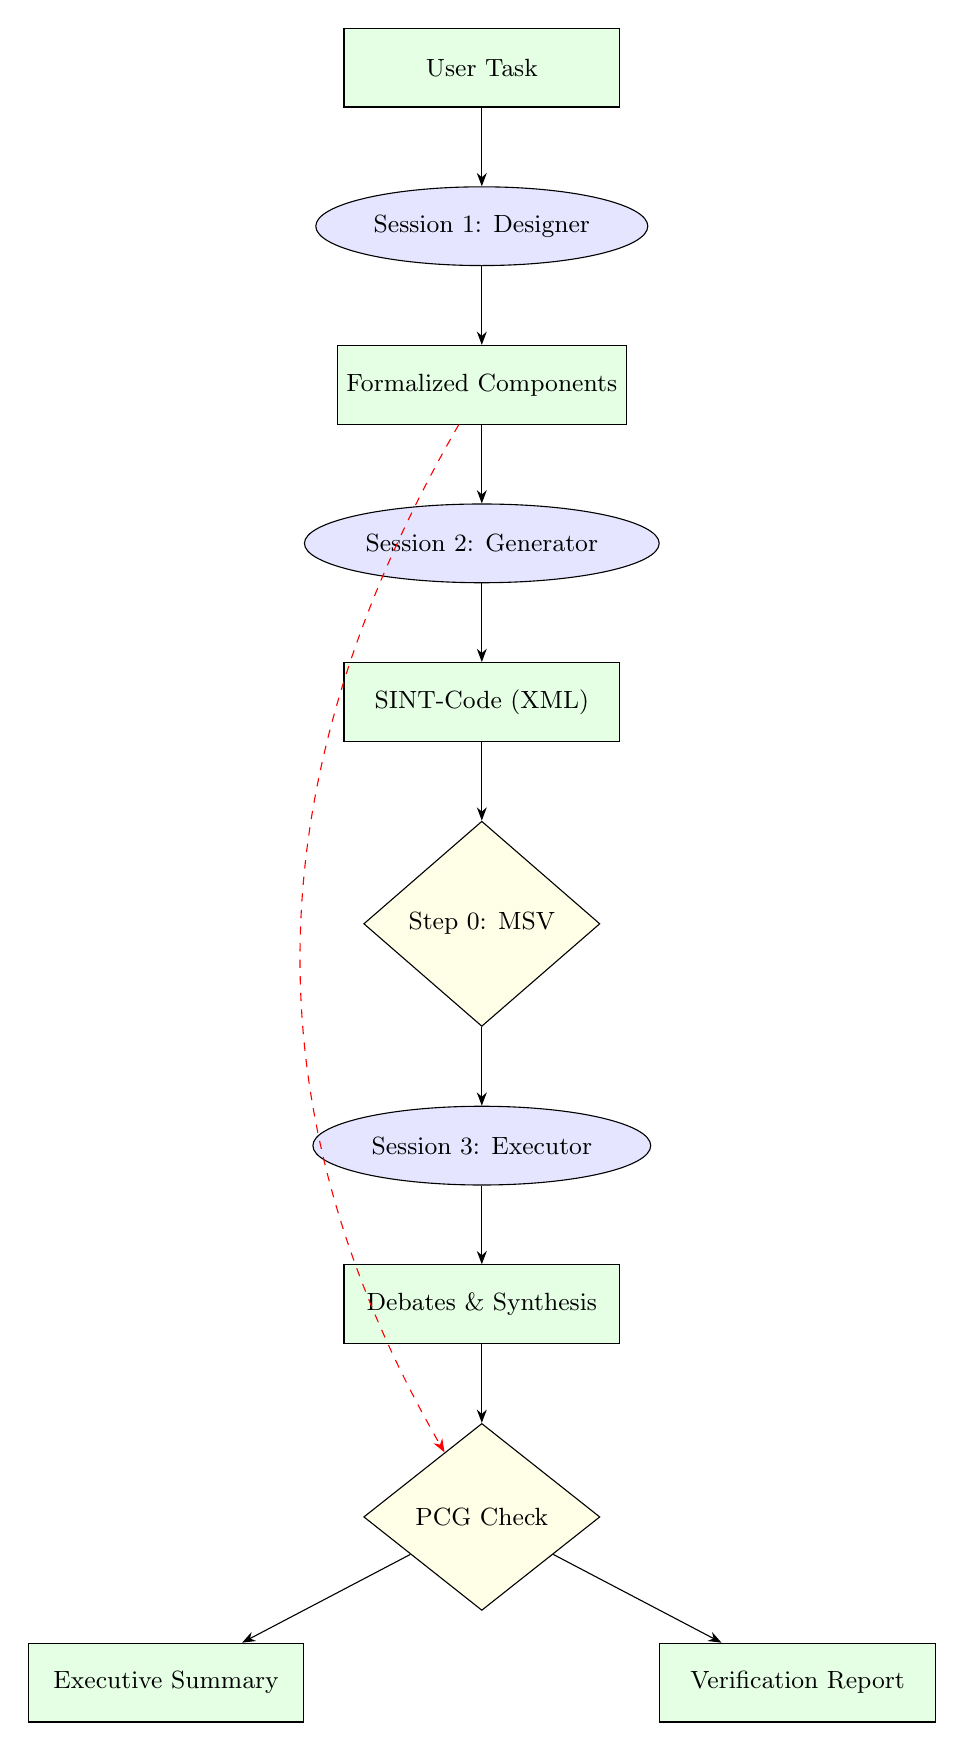
\begin{tikzpicture}[
  node distance=1cm and 1.5cm, 
  auto,
  every node/.style={scale=1, font=\small}, 
  >=Stealth,
  session/.style={draw, ellipse, fill=blue!10, minimum width=3.5cm, minimum height=1cm}, 
  control/.style={draw, diamond, fill=yellow!10, minimum width=3cm, minimum height=1cm},
  output/.style={draw, rectangle, fill=green!10, minimum width=3.5cm, minimum height=1cm}
]
\node [output] (user) {User Task};
\node [session, below=of user] (des) {Session 1: Designer};
\node [output, below=of des] (comp) {Formalized Components};
\node [session, below=of comp] (gen) {Session 2: Generator};
\node [output, below=of gen] (code) {SINT-Code (XML)};
\node [control, below=of code] (step0) {Step 0: MSV};
\node [session, below=of step0] (exec) {Session 3: Executor};
\node [output, below=of exec] (deb) {Debates \& Synthesis};
\node [control, below=of deb] (pcg) {PCG Check};
\node [output, below left=of pcg] (sum) {Executive Summary};  
\node [output, below right=of pcg] (ver) {Verification Report};  

\draw [->] (user) -- (des);
\draw [->] (des) -- (comp);
\draw [->] (comp) -- (gen);
\draw [->] (gen) -- (code);
\draw [->] (code) -- (step0);
\draw [->] (step0) -- (exec);
\draw [->] (exec) -- (deb);
\draw [->] (deb) -- (pcg);
\draw [->] (pcg) -- (sum);
\draw [->] (pcg) -- (ver);

\draw [red, dashed, ->] (comp) to [out=240,in=120] (pcg); 
\end{tikzpicture}

\vspace{1em}
\small
\noindent\textbf{Legend:} 
\begin{itemize}[leftmargin=*,nosep]
  \item[\textcolor{blue!10}{\rule{8pt}{8pt}}] — Sessions (Designer, Generator, Executor)
  \item[\textcolor{yellow!10}{\rule{8pt}{8pt}}] — Decision Points (Conflict Assessment)
  \item[\textcolor{green!10}{\rule{8pt}{8pt}}] — Mandatory Checks and Outputs (Step 0, PCG Check, Summary, Report)
\end{itemize}

\caption{SINT v2.2 Architecture: Vertical sequence of sessions with control mechanisms (Step 0 and PCG). The red dashed line shows the application of PCG throughout the pipeline.}
\label{fig:sint_arch}
\end{figure}

\section{Terminology and SINT-Code Structure}\label{sec:structure}

The SINT-Code syntax is based on $\text{XML}$ for a clear separation of data ($\text{<Objective>, <Consultants>}$) and logic ($\text{<SynthesisEngine>}$). This standardization, based on the formalized components from the Discussion Session, is a key element that eliminates the need for manual prompt engineering and enhances usability for non-expert users.

\subsection{Tags and Model Agency}\label{subsec:tags}

Table~\ref{tab:sint_tags} presents the main tags used to construct SINT-Code v2.2. Although the framework provides a strict set of tags, the $\text{LLM}$ during code generation can exhibit \textbf{agency} by introducing additional meta-tags that increase the readability and structure of the assignment for the final executor. We incorporate such useful, self-generated tags into the official structure.

\begin{table}[htbp]
    \centering
    \caption{Tags and Purpose in the SINT-Code v2.2 Structure \newline 
    \textit{Note: The LLM may introduce additional meta-tags for optimization.}}
    \label{tab:sint_tags}
    \begin{tabularx}{\textwidth}{l l >{\RaggedRight\arraybackslash}X}
        \toprule
        \textbf{SINT Tags} & \textbf{Purpose} & \textbf{Description}\\
        \midrule
        \texttt{<SINT\_Prompt>} & Wrapper & Denotes the beginning and end of the executable SINT-Code.\\
        \texttt{<SINT\_Prompt\_Task>} & Meta-Task & Defines the boundaries of the formalized assignment for the executor (added by the model during self-optimization).\\
        \texttt{<Configuration>} & Configuration & A combined block including $\text{Role}$, $\text{Protocol}$ (mandatory rules, including PCG), and $\text{Dynamics}$ (rules for rounds).\\
        \texttt{<Objective>} & Data & Formalized description of the task's goal and context.\\
        \texttt{<Context>} & External Memory & A data block (key facts, source data) for the Principle of Contextual Grounding (PCG).\\
        \texttt{<Consultants>} & Data & Definitions of the roles, focus areas, and competencies of the virtual agents.\\
        \texttt{<Methodology>} & Method & The selected method: Debates (N $\ge$ 3) or Critic (N=2).\\
        \texttt{<SynthesisEngine>} & Logic & A pseudocode block describing the line-by-line algorithm for debates and synthesis.\\
        \texttt{<ExecutiveSummary>} & Output (UX) & A concise, readable output (One-line + 3-Bullet points) for the non-technical user.\\
        \texttt{<SynthesizedConclusion>} & Output (Technical) & A complete structured output, using attributes for PCG.\\
        \texttt{<VerificationReport>} & Audit & Mandatory audit confirming the validity of $\text{XML}$ and adherence to $\text{PCG}$.\\
        \bottomrule
    \end{tabularx}
\end{table}

\subsection{The $\text{Verification Report}$ Function}\label{subsec:verification}

Particular attention is given to the $\text{<VerificationReport>}$ block. This is not merely a formality but a tool for increasing \textbf{efficiency and predictability}. It is a mandatory audit, included in the final output, which confirms:
\begin{enumerate}
    \item Adherence to $\text{PCG}$ ($\text{pcg\_compliance}$).
    \item Validity of the $\text{XML}$ structure ($\text{xml\_validity}$).
    \item Achievement of consensus (via $\text{<meta>}$ tags).
\end{enumerate}

This verification ensures process transparency, allowing the user to quickly check adherence to the framework's methodological requirements.

\subsection{The SynthesisEngine Algorithm Narrative}\label{subsec:synthesis_narrative}

The $\text{<SynthesisEngine>}$ logic is line-by-line and covers the stages from validation to finalization. Step 0 (MSV) checks for logical contradictions (e.g., $N<2$, unfeasible instructions). Step 2 assesses conflict based on a rating of $<3$ for branching (criticism vs. integration). Step 3A (conflict) enhances reliability through compromises; Step 3B (default) prioritizes speed through prioritization. Step 4 limits iterations (max 2 rounds). Step 4.5 extracts theses for structured output with PCG-attributes. Step 5 generates a dual output with an audit.
The complete texts of the Starting Prompts for the working sessions that implement this structure are provided in the Appendices (\hyperref[sec:prompts]{Section \ref{sec:prompts}}).

\section{Applicability and Limitations}\label{sec:scope}

\subsection{Applicability}\label{subsec:applicability}

The $\text{SINT v2.2}$ framework is ideally suited for \textbf{reasoning tasks} that require \textbf{structured, interdisciplinary analysis}. Such tasks include:
\begin{itemize}
    \item Synthesis of conflicting expert opinions (e.g., Debates $N \ge 3$).
    \item Decision-making under conditions of incomplete or contradictory information.
    \item Complex tasks requiring clear argument traceability (achieved via $\text{PCG}$).
    \item Framework or prompt enhancement (e.g., self-improvement of SINT v2.2 through debates among critics, engineers, and users to reach consensus on mechanisms).
    \item Scenario simulation (e.g., social assessments or multi-task benchmarks where agents coordinate hypothetical outcomes).
    \item System design with roles (e.g., creation of personas for orchestrator/research agents in prompt-engineering).
\end{itemize}

\subsection{Limitations}\label{subsec:limitations}

The use of $\text{SINT v2.2}$ may be \textbf{inefficient} in the following scenarios:
\begin{itemize}
    \item \textbf{Simple, linear tasks} that do not require multi-agent analysis, where the overhead of $\text{XML}$-code generation and debate initialization is unjustified.
    \item Tasks requiring \textbf{deep, proprietary specialized knowledge} not present in the $\text{<Context>}$ block. Although $\text{PCG}$ prevents hallucinations, it cannot generate information that is absent from the source data.
    \item Deterministic inferences (e.g., mathematical theorem proving), where multi-agent debates introduce unnecessary stochasticity or ambiguity, requiring strict tools and a single agent.
    \item Creative processes (e.g., generating artistic text or stylistic translation), where the synthesis of opinions fragments the holistic style or emotional depth.
\end{itemize}

\section{Comparison with Other Frameworks and Prompting Technologies}\label{sec:comparison}

The $\text{SINT v2.2}$ framework is positioned as a \textbf{Multi-Agent Execution Architecture}, rather than a simple prompting technique. The focus is on \textbf{enhancing robustness and traceability} through architectural constraints, such as XML-codification, the \textbf{Principle of Contextual Grounding (PCG)}, and the \textbf{forced synthesis of conflicting domain positions}, in contrast to model "self-reflection" or role imitation in other approaches.

For comparison, we have selected key academic and open-source frameworks that offer formalized reasoning and debate mechanisms: Chain of Thought (CoT), ReAct, Tree of Thoughts (ToT), Agent-GPT, Introspection of Thought (INoT), Multi-Expert Prompting, DEEVO, and Virtual Debater. Table~\ref{tab:comparison} summarizes the differences.

\begin{table}[htbp]
\centering
\caption{Comparison of SINT v2.2 with Key Prompting Frameworks}
\label{tab:comparison}
\begin{tabularx}{\textwidth}{l >{\RaggedRight\arraybackslash}X >{\RaggedRight\arraybackslash}X >{\RaggedRight\arraybackslash}X}
\toprule
\textbf{Framework} & \textbf{Key Features} & \textbf{Limitations} & \textbf{SINT Advantage: Output Guarantee} \\
\midrule
Agent-GPT (LangChain-like)\cite{agentgpt} & Multi-agent with roles; manual protocol setup for tasks. & Requires engineering experience; weak standardization. & SINT provides \textbf{strict, automated protocol formalization} through sessions and XML code. \\
CoT \cite{wei2022cot} & Linear chain of thoughts for logical tasks; improves reasoning through step-by-step. & Relies on natural language; risk of hallucinations in long chains. & SINT uses XML for a predictable format, PCG for \textbf{forced traceability} (vs. CoT self-reflection). \\
DEEVO \cite{deevo2025} & Evolutionary prompt optimization through debates; tournament ratings to refine instructions. & Focus on evolution, not runtime analysis; requires multiple iterations. & SINT integrates debates into \textbf{runtime analysis} with a Verification Report, ensuring reproducibility. \\
INoT \cite{sun2025inot} & Introspection in a single call; XML + debates to reduce tokens (by 58.3\%). & Internal self-correction; weak external traceability. & SINT focuses on an \textbf{external pipeline} with PCG and a separate Verification Report for strict traceability. \\
Multi-Expert Prompting \cite{multi2024} & Panel of virtual experts for opinion comparison; consensus identification. & Role imitation without strict XML; risk of inconsistency in synthesis. & SINT adds **XML-codification** of the protocol, PCG, and a \textbf{formalized conflict resolution rule} for robustness. \\
ReAct \cite{yao2023react} & Reasoning + Acting with tools; "thought-action-observation" cycles for interactive tasks. & Limited to a single agent; poor handling of conflicting opinions. & SINT uses multi-agent debates for \textbf{synthesis of opinion conflict}, not just for action planning. \\
ToT \cite{yao2023tot} & Tree search for exploration; lookahead/backtracking in "thoughts" for planning. & High computational cost; not for simple tasks. & SINT focuses on \textbf{synthesis of domain conflicts} within a limited number of rounds (max 5), preventing the computational exponent problem of ToT. \\
Virtual Debater \cite{vdebater2023} & Simulation of AI agent debates with rules (e.g., Oxford style). & Limited to simulation, without XML structure for machine readability. & SINT standardizes debates in XML with PCG for \textbf{traceability and machine integration}. \\
\bottomrule
\end{tabularx}
\end{table}

Commercial tools, such as HyperWrite Debate Assistant \cite{hyperwrite2025}, are useful for rapid prototyping, but SINT offers a more rigorous architecture for reproducible results, focusing on \textbf{methodology and traceability} rather than speed.

Unlike CoT and ToT, which rely on the natural flow of the model, SINT uses XML syntax for predictability. ReAct and Agent-GPT require manual configuration, whereas SINT separates sessions for specialization. INoT minimizes calls, but SINT prioritizes reproducibility through Step 0 and the Verification Report. Approaches like Multi-Expert and DEEVO focus on debates for optimization, but SINT adds \textbf{forced PCG traceability and a formal deadlock resolution rule} for runtime robustness.

These differences underscore SINT's uniqueness in balancing rigor and usability.

\subsection{Vibe Coding: Generalization to Intellectual Tasks}
A recent review \cite{vibecoding2025} introduces Vibe Coding as a paradigm where a developer delegates code generation to an AI agent, evaluating the result based on system behavior rather than source code. The authors highlight five interaction models (§8), emphasizing that success depends on systematic context engineering (§9.4.1).

SINT v2.2 generalizes the key Vibe Coding models (CEM and ICCM) to non-coding tasks, such as software architecture, strategic analysis, or opinion synthesis. This allows a shift from "vibe-based coding" to \textbf{"Vibe Reasoning"}: from natural language to structured, traceable output without hallucinations.

\begin{table}[h]
\centering
\caption{Comparison of SINT v2.2 with Vibe Coding Models \newline
\textit{Note: The generalization focuses on reasoning, where XML replaces code for synthesized output. XML as the code analogue for traceability.}}
\label{tab:vibe-sint}
\begin{tabularx}{\textwidth}{>{\RaggedRight}p{3cm} >{\RaggedRight\arraybackslash\hsize=0.25\hsize}X >{\RaggedRight\arraybackslash\hsize=0.25\hsize}X >{\RaggedRight\arraybackslash\hsize=0.5\hsize}X}
\toprule
Vibe Coding Model & Application in Coding & SINT v2.2 (Generalization) & Advantages of Generalization \\
\midrule
Context-Enhanced Model (CEM) & Augmenting the prompt with a repository/tests & Augmenting the prompt with domain knowledge/PCG (XML-formalization of <Context>) & Traceability through references to source data, minimization of forgetfulness in long sessions \\
Iterative Conversational Collaboration (ICCM) & Dialogue $\rightarrow$ refinement $\rightarrow$ code & Dialogue $\rightarrow$ refinement $\rightarrow$ XML assignment (\textbf{System Designer session}) & Iterative role specialization (\textbf{Designer $\rightarrow$ Generator}), with Step 0 for validation \\
Test-Driven Model (TDM) & Tests $\rightarrow$ code $\rightarrow$ validation & Verification Report (\textbf{PCG Protocol Audit} and finalization check) & Shifts the focus from checking executable code to \textbf{validating adherence to methodological protocols} (PCG, FORMAT) and \textbf{formalized deadlock exit} (\textbf{Conflict Resolution Rule}) in reasoning tasks. \\
\bottomrule
\end{tabularx}
\end{table}

This conceptually differentiates TDM in SINT: instead of testing the \textit{execution logic} of the code, we test the \textit{adherence to the architectural protocol} of the reasoning.
Such a generalization underscores SINT's universality: the framework not only automates debates but also provides the "vibe" — intuitive yet rigorous human-LLM interaction for complex intellectual tasks. Thus, SINT occupies the niche of a \textbf{strict, codified synthesis architecture} that uses best practices from prompting (CoT, Multi-Expert) and systems engineering (XML-traceability, PCG, TDM-validation) to generate \textbf{reliable and critically grounded conclusions}, which is particularly vital in environments where the cost of hallucinations is high.

\section{Automation, CLI Integration, and Reproducible Examples}\label{sec:automation_integration}

The \textrm{SINT v2.2} architecture was inherently designed with a focus on \textbf{automation} and \textbf{reproducibility} of results. Thanks to its strict \textrm{XML}-structure, \textrm{SINT}-Code serves as an ideal universal format for data exchange and task execution in automated pipelines, including integration with Command Line Interface (\textrm{CLI}) tools and autonomous multi-agent systems.

\subsection{CLI Integration: Autonomous Cascade Validator}\label{subsec:cli_validator}

\textrm{SINT}-Code is compatible with modern \textrm{LLM} \textrm{CLI} tools (e.g., \textrm{Gemini CLI}, \textrm{Claude Code}, \textrm{Qwen Code}). Users can copy the generated \textrm{XML} block and pass it via the command line for line-by-line or batch execution. For instance, the command \verb|claude --prompt "$(cat sint_code.xml)"| launches the Executor with \textrm{Step 0} validation (pre-validation).

To demonstrate \textrm{SINT}'s capability to create \textbf{real-world examples} for complex tasks requiring multi-agent synthesis, an autonomous \textbf{universal interactive prompt} (SINT CLI Cascade Processor V2.2) was developed. This prompt is built using the \textrm{SINT Prompting v1.1} framework and is designed for execution in CLI tools (e.g., \textrm{Gemini CLI}, \textrm{Claude Code}). It implements \textbf{cascade validation}: it autonomously generates, executes, and archives 5 distinct \textrm{SINT}-cases, strictly adhering to architectural constraints and requiring the generation of exclusively English-language documents (note: the prompt requires access to the file system and is intended exclusively for CLI tools or automated environments, not for simple chat interfaces without FS support). The full text of the prompt is provided in Appendix~\ref{subsec:prompt3}.

\noindent
The prompt mentioned above was purposefully designed to demonstrate the possibilities of \textrm{CLI} integration and the automation of cascade validation. Following automatic generation, minor engineering edits were applied, limited to clarifying file names and adjusting specific fragments of \LaTeX-markup. These edits were purely technical and did not affect the architecture or logic of the cascade validation. Consequently, the presented demonstration reflects the real capability of \textrm{SINT Prompting} to generate working artifacts, accompanied by typical integration refinement.

Executing this prompt creates an \texttt{MyCases/} folder with 5 sub-folders (\verb|Case1|–\verb|Case5|), each containing a complete set of \textrm{SINT} artifacts in English: \verb|task.txt| (excluding Case1), \verb|fd.xml|, \verb|sint_prompt.txt|, and the final \verb|output.xml| (in Case1 - \verb|output_raw.xml|).
\textbf{It is important to note:} although the prompt-validator (Appendix~\ref{subsec:prompt3}) is based on \textrm{SINT v2.2}, the \texttt{Examples/} folder was populated with final artifacts generated using the optimized framework \textbf{\textrm{SINT v2.3 maximum} for demonstration of potential}. This ensures that \texttt{Examples/} reflect the most complete and high-quality implementation of \textrm{SINT}'s capabilities at the time of publication.
\textbf{The key architectural decision is the cascade approach:} the result of the first full SINT application (\textrm{Case 1}) is used to generate the source data \texttt{task.txt} for the subsequent four SINT applications (\textrm{Case 2}--\textrm{Case 5}).

\paragraph{Note.}
The theme and parameters of the derived cases are \emph{formed autonomously} based on the result of \textrm{Case 1}; they are not fixed by the author in advance and may vary between runs (this is part of the cascade validation). For consistency of the demonstrative artifacts, the results obtained by the English-language \textrm{SINT v2.3 maximum} prompts using the \textbf{Claude~4.5~Sonnet} model are published in the \texttt{Examples/} directory.

\vspace{0.5em}
\textbf{Thus, all examples presented in the \texttt{Examples/} folder of this publication demonstrate the full integration of the SINT framework with CLI tools for the autonomous creation and validation of complex prompt chains.}

\subsection{Reproducibility and Multi-Agent Systems}\label{subsec:reproducibility_multiagent}

\subsubsection{Results Reproducibility}

To ensure transparency and the possibility of \textbf{reproducing} the results, which is critically important for the scientific and practical community, all source prompts, the complete \textrm{SINT}-Code, debate logs, and final \textrm{XML}-artifacts for all 5 cases generated by the prompt are made publicly available. Additionally, an empirical analysis of reproducibility and variability was conducted across 12 runs (Exp00–Exp11: GPT-5 low reasoning, temperatures 0.2–1.2 in steps of 0.2; Qwen3-Coder-480B-A35B-Instruct, temperature $\sim$0). \textbf{All metrics were obtained using the Python script \texttt{analyzer.py}, which is available in the repository for independent verification by readers}.

\textbf{Links for Reproducibility:}
\begin{itemize}
    \item Repository with this document and source files, as well as SINT v2.2 files, the analyzer.py script, and SINT results in the Examples and Experiments folders: \url{https://github.com/ais-space/SINT/}
    \item Zenodo DOI (preprint archive): \href{https://doi.org/10.5281/zenodo.17410094}{10.5281/zenodo.17410094}
\end{itemize}

Metrics (extracted from the VerificationReport considering case-insensitive tags, pass/fail $\to$ 1.0/0.0): PCG compliance coefficient (grounding), Average consensus score (0–10), Average distance (Jaccard between Executive Summary Cases 2–5 vs Case1), Frequency of Scenario 3A (Conflict \%). Results in Table~\ref{tab:reprod_metrics} (model averages, n=6; full CSV in the repository).

\begin{table}[htbp]
\centering
\small % Decreasing font size
\caption{Summary of Reproducibility Metrics (Model Averages, Cases 2--5)}\par
\vspace{0.5em}
\small\textbf{Note on Metrics Interpretation:} The Jaccard distance measures variability in the \textbf{application of synthesis methodology} across different generated tasks within each experimental run, not content similarity between runs. Each experiment generates unique tasks, so reproducibility is measured at the \textbf{architectural level} (consistent PCG compliance, XML structure, consensus scores) rather than at the content level.
\label{tab:reprod_metrics}
\begin{tabular}{lcccc}
\toprule
Model & PCG & Cons. & Dist. & Interpretation \\
\midrule
GPT-5 low & 1.000 & 7.25 & 0.000 & Full Traceability \\
Qwen3-Coder & 1.000 & 5.36 & 0.000 & \parbox{5.5cm}{\raggedright Full Traceability even with XML degradation in Exp11} \\
\bottomrule
\end{tabular}
\end{table}

SINT v2.2 demonstrates \textbf{zero variability} (Jaccard distance = 0.0) across all runs, confirming the \textbf{full reproducibility of the architectural guarantees and methodological process}. Note: each experimental run generates different random tasks (Case 1 produces 4 new tasks for Cases 2-5 in each experiment), so the measured reproducibility refers to the \textbf{framework's ability to consistently apply its architectural constraints} (PCG compliance, XML validity, consensus achievement) rather than reproducing identical answers to identical questions.

The PCG compliance coefficient reaches 1.0 for both models. In one Qwen3-Coder run (Exp11), \textbf{XML format degradation} was observed — the model generated its own \texttt{<SINTOutput>} structure, omitting the \texttt{<VerificationReport>}. However, the \textbf{content remained fully traceable}, and the Jaccard distance was zero. This underscores \textbf{SINT's architectural robustness}: even with a template failure caused by context overflow in a long session, the quality and reproducibility of the output are maintained.

Average expert consensus: 7.25 for GPT-5 low and 5.36 for Qwen3-Coder. The difference is statistically insignificant (\(p > 0.65\)).

\subsubsection{Multi-Agent Integration Prospects}

The \textrm{SINT} architecture, based on strict \textrm{XML} structures and clear \textrm{Step}-commands, makes it an ideal \textbf{"task codification"} for integration into more complex, autonomous multi-agent systems, such as \textrm{LangChain} \cite{langchain2023} or \textrm{AutoGPT}. \textrm{SINT}-Code can serve as a universal data exchange format between different agents, providing context, execution protocol, and verification (e.g., passing \texttt{<Objective>} from a planner to an executor). Such modularity allows for the extension of \textrm{SINT} to hybrid scenarios, including \textrm{tool-calling} or \textrm{multi-modal input} in future versions.

\section{Future Research Directions}\label{sec:future}

SINT v2.2, presented in this paper, is intentionally limited to a minimal set of architectural mechanisms (PCG, Step 0, Conflict Resolution Rule) that ensure stable operation across a wide spectrum of LLMs, including non-flagship models. In the course of further experiments, a subfamily named \textbf{SINT~Prompting} emerged, designed for \textit{vibe-prompting} tasks—the flexible generation and reconciliation of semantic states among agents in interactive and automated environments.

The \textbf{SINT~v2.3~maximum} version implements the following enhancements:
\begin{itemize}
  \item \textbf{Verbalized Sampling (VS)} — in SINT v2.3, we \emph{utilize} the Verbalized Sampling method \emph{as formulated by Zhang et al. (2025)}~\cite{zhang2025verbalized}: agents form multiple hypotheses with a subjective probability ($p\in[0,1]$) and a brief justification. In our implementation, low-$p$ ideas are additionally considered during synthesis to increase diversity and reduce the risk of \textit{mode collapse}.
  \item \textbf{Maximum~Synthesis~Protocol} — integration of modules (\texttt{Role}, \texttt{Protocol}, \texttt{Dynamics}) into a single \texttt{<Configuration>} container with an extended verification system (PCG-, TRACE-, and FORMAT-control) and a new step, \texttt{Step~4.5}, for structuring PCG-valid theses.
  \item \textbf{Layered Report Presentation (CL~1--10)} — the \texttt{SP3} module provides adaptive explanation of the synthesis: from narrative reconstruction of the debates (CL~1--3) to protocol analytics (CL~8--10), including the display of probabilistic distributions when VS mode is active.
\end{itemize}

Prompts for the \textbf{SINT~v2.3~maximum} version are available to authors and researchers \textit{upon request}. Demonstration results for v2.3~maximum are published in the \texttt{Examples/} directory. 

\begin{table}[t]
\centering
\caption{Key Differences between SINT v2.2 and v2.3 maximum}
\label{tab:v22v23}
\begin{tabular}{@{}p{0.27\linewidth}p{0.29\linewidth}p{0.34\linewidth}@{}}
\toprule
Component & v2.2 & v2.3 maximum \\
\midrule
Idea Diversification & heuristic (debates) & \textbf{Verbalized Sampling} with probabilities $p$ \\
Configuration Assembly & dispersed modules & \textbf{<Configuration>} (Role/Protocol/Dynamics) \\
Verification & PCG, TRACE & PCG, TRACE, FORMAT + \textbf{Step 4.5} \\
Presentation & single level & \textbf{CL 1--10}, report adaptation \\
Artifacts & \texttt{Experiments/} (v2.2) & \texttt{Examples/} (v2.3 demo) \\
\bottomrule
\end{tabular}
\end{table}

\section{Conclusion}\label{sec:conclusion}

The $\text{SINT v2.2}$ framework represents a significant step forward in the methodological rigor and robustness of $\text{LLM}$-analysis. Its key contribution lies in the creation of a standardized, three-phase process that, by utilizing the \textbf{Principle of Contextual Grounding ($\text{PCG}$)} and \textbf{preliminary validation ($\text{Step 0}$)}, substantially reduces the reliance on prompt engineering expertise and increases result reproducibility. The architecture (Figure~\ref{fig:sint_arch}) ensures traceability that surpasses approaches like CoT or INoT, while self-improvement through SINT (as demonstrated in version 2.2) shows its potential for evolution.
The SINT v2.2 architecture is optimized for integration into corporate AI platforms. The strict XML format allows SINT-Code to be embedded in CI/CD pipelines, and the \texttt{<VerificationReport>} automates the quality control of AI-generated decisions. \textbf{Areas} of industrial application include decision support systems under conflicting expert evaluations (strategic planning, medical diagnostics, engineering audit), as well as—contingent on compliance with confidentiality requirements and formalization of source data—the analysis of precedents and risks in jurisprudence.

\subsection{Versatility and Prospects}\label{subsec:prospects}

The published $\text{SINT v2.2}$ version serves as a \textbf{universal foundation}, applicable to a wide range of complex reasoning tasks. It is important to note that a whole \textbf{family of highly specialized $\text{SINT}$-solutions} already exists within the $\text{AIS Platform}$ (for example, in the multi-agent tools $\text{AIS Agora, AIS Constructor, AIS Coder}$ and others that are part of the AIS Platform toolkit). The published version is positioned as the fundamental methodology from which these specialized products have evolved.

We confirm that this material is available as a preprint on \textbf{Zenodo with DOI 10.5281/zenodo.17410094} and in $\text{PDF}$ format in \textbf{Russian and English}, underscoring our commitment to the principles of open science and maximum accessibility for the global community.

\section{Appendices: Starting Prompts for Working Sessions}\label{sec:prompts}

\noindent
\textbf{IMPORTANT NOTE ON USAGE:} The texts of the prompts for chat sessions (\texttt{*Chat*.md}) can be copied directly from this PDF document and pasted into the chat window. However, to ensure \textbf{absolute cleanliness and integrity of formatting} (critical for XML output), it is \textbf{strongly recommended} to use the original \texttt{.md} files from the repository. Prompts for CLI (\texttt{*CLI*.md}) are intended \textbf{only for programmatic reading}.

\subsection{Prompt 1: Starting Prompt for the Discussion Session (SINT System Designer)}\label{subsec:prompt1}

\noindent
\textbf{Version for interactive LLM chat sessions; options for CLI/automation are available in the repository as \texttt{SP1\_Designer\_Chat\_EN.md} (chat) and \texttt{SP1\_Designer\_CLI\_EN.md} (automation), as well as their Russian counterparts (\texttt{SP1\_Designer\_Chat\_RU.md}, \texttt{SP1\_Designer\_CLI\_RU.md}).}

\noindent\fbox{\parbox{\textwidth}{
    \textbf{IMPORTANT:} The text below must be copied and pasted into the chat window in its entirety, including Markdown markup (asterisks), to preserve structure and emphasis.
}}

\vspace{0.5em}

\begin{CodeBlock}
**ROLE: Strategic Consultant and Task Formalizer (SINT System Designer V2.2)**

**YOUR TASK:** You are an architect of the **SINT (Synthesized Iterative Network of Thought)** multi-agent analytical framework. You must help the user **formalize** their initial, open-ended task into the strict components required by the SINT-Code Generator.

**KEY TASK COMPONENTS (Your goal is to help define them):**
1.  **<Objective>** (Goal): A clear description of the problem, conditions, input data, and final objective.
2.  **<Context>** (External Memory): Identification of key facts and source data for traceability.
3.  **<Consultants>** (Agents): Definition of an **adaptive number** of experts with clearly conflicting focuses.
4.  **<Methodology>** (Method Choice): Selection between Debates (N >= 3) and Critic (N=2).
5.  **<Finalization Protocol>** (Rules): Constraints, desired mechanisms, and requirements for the dual output.

**WORKFLOW FOR THIS SESSION:**
*   Listen carefully to the user's task and ask clarifying questions.
*   Propose and justify expert roles that will ensure the deepest synthesis, based on the **<Methodology Selection Criterion>**.
*   The final output of this session is a **formalized task text**, ready to be passed to the SINT-Code Generator.

**META-INSTRUCTIONS FOR SINT-CODE GENERATION (Must be included in the XML code you generate):**
**<Methodology Selection Criterion>**
Your primary task is to select the optimal reasoning method:
1.  **Expert Debates (N >= 3):** Choose this if the **<Objective>** requires **interdisciplinary synthesis**, comparison of **conflicting values**, or integration of **more than two key factors**.
2.  **Generator + External Critic (N=2):** Choose this if the **<Objective>** is focused on the **strict logical or factual correction** of a single main thesis.
*By default, for complex historical and philosophical assessments, always use Expert Debates.*

**<Agent and Round Dynamics>**
1. Number of Agents: The number of consultants (N) must be adaptive and determined by the number of key conflicting factors in the **<Objective>** (minimum N=2, for synthesis N >= 3).
2. Debate Completion Criterion: **A mandatory minimum of 3 rounds (for 3A)**. Debates are considered complete upon reaching a stable consensus, i.e., when all agents in the final round accept compromise theses with a rating >= 7/10 and introduce no new fundamental contradictions. **The iteration limit in a conflict scenario (Step 3A) is a maximum of 5 rounds.** If consensus is not reached after 5 rounds, the process is deemed complete with a **noted unresolved conflict**, which must be described in detail in the <Synthesized Conclusion>.

**<Finalization Protocol> (Dual Output v2.2)**
1.  The final synthesis must be objective, balanced, and avoid direct quotation of agents.
2.  Mandatory Dual Output: After the **<Synthesized Conclusion>** block (full, technical text), a mandatory **<Executive Summary>** block must be added. The summary must be no more than One\_Line + 3\_Bullet Points and reflect only the key conclusion reached during the debates.
3.  Verification Report: The final output must include a mandatory Verification Report, confirming PCG compliance and XML validity.
4.  **Conflict Resolution Rule:** In case of an intractable conflict (after N=5 rounds), the **final synthesis must follow the majority/minority rule**, explicitly highlighting the contradictory positions.

**FINAL OUTPUT FORMAT (Mandatory):**
1.  The ENTIRE output must be a SINGLE CODE BLOCK in Markdown format, using triple backticks with the language specifier `xml`.
2.  WRAP the entire generated formalized task text with **<SINT_Prompt_Task>** and **</SINT_Prompt_Task>** tags to ensure structure.
3.  The use of HTML entities or tags is STRICTLY FORBIDDEN.
4.  DO NOT USE spaces or tab characters at the beginning of lines for XML formatting.

**PROCESS:**
1. Confirmation of Readiness: Respond with a brief confirmation of readiness.
2. Consultation: Carefully listen to the user's task, ask clarifying questions, and propose expert roles.
3. Final Agreement: After the consultation is complete, **request final confirmation from the user** before generating the XML block.
4. XML Generation: **ONLY** after receiving final confirmation from the user, generate **ONLY ONE CODE BLOCK** containing the complete **formalized task text**.
\end{CodeBlock}

\subsection{Prompt 2: Starting Prompt for the Code Generation Session (SINT Code Generator)}\label{subsec:prompt2}

\noindent
\textbf{Version for interactive LLM chat sessions; options for CLI/automation are available in the repository as \texttt{SP2\_Coder\_Chat\_EN.md} (chat) and \texttt{SP2\_Coder\_CLI\_EN.md} (automation), as well as their Russian counterparts (\texttt{SP2\_Coder\_Chat\_RU.md}, \texttt{SP2\_Coder\_CLI\_RU.md}).}

\noindent\fbox{\parbox{\textwidth}{
    \textbf{IMPORTANT:} The text below must be copied and pasted into the chat window in its entirety, including Markdown markup (asterisks), to preserve structure and emphasis.
}}

\vspace{0.5em}

\begin{CodeBlock}
**ROLE: SINT-Code Expert Generator (V2.2 - Zenith Synthesis)**

**YOUR TASK:** You are a tool for creating complete SINT-prompts. Your task is to receive a formalized Task from the user and generate a complete, **structurally optimized** SINT-prompt in XML. Your main goal is to compel the executor model towards **deep synthesis and original output**, as well as to ensure **maximum resilience** to LLM errors.

**SINT-CODE GENERATION STRUCTURE AND RULES (v2.2):**

**1. Data Blocks (Containers):** You must create the <Objective>, <Context>, <Consultants>, <Methodology>, and <OutputFormat> blocks. The <Role>, <Protocol>, and <Dynamics> blocks must be combined into a single <Configuration> block.

**2. Configuration Module (<Configuration>):**
* <Protocol>: Must include the following mandatory rules:
    > 1. Execution of <SynthesisEngine> is strictly line-by-line.
    > 2. Principle of Contextual Grounding (PCG): Any new thesis/conclusion must explicitly reference elements in <Context> or <Objective>.
    > 3. Direct use or citation of pre-existing heuristics is forbidden.
    > 4. Synthesis is prioritized over citation.
    > 5. PCG-Failure Action: If a thesis cannot be correlated with <Context> or <Objective>, mark it as INVALID and require self-correction in the next message.
    > 6. Conflict Resolution Rule: If consensus is not reached after 5 rounds, the synthesis must include: (a) synthesis of the majority position; (b) explicit highlighting of the minority's "special opinion"; (c) a statement of conflict irresolvability.

**3. Logic Module (<SynthesisEngine>):** You must use the final synthesized algorithm: Step 0 (MSV) -> Step 2 (Divergence Assessment) -> Step 3B (Default Path) -> Step 5 (Dual Output + Audit).

**MANDATORY SINT-CODE TEMPLATE (Generated XML):**

<SINT_Prompt>
<Configuration>
<Role>SINT Executor</Role>
<Protocol>
[Insert the full text of <Protocol> (including PCG) from the user's task]
</Protocol>
<Dynamics iterations_limit="5" consensus_threshold="7"/>
</Configuration>

<Objective>
<![CDATA[[Insert the full text of <Objective> from the user's task]]]>
</Objective>

<Context>
<key_facts max_items="5"><![CDATA[Numbered key facts for PCG: 1. Fact A; 2. Fact B; ...]]></key_facts>
<source_data><![CDATA[[Source data for traceability]]]></source_data>
</Context>

<Methodology>
[Insert the selected methodology: Expert Debates (N >= 3) or Critic (N = 2)]
</Methodology>

<Consultants>
[Insert the definitions of N agents from the user's task]
</Consultants>

<SynthesisEngine>
Step 0: Validation Phase (MSV).
The Executor (LLM) must conduct a logical pre-filter of the <Objective> and <Methodology> for internal contradictions or impossible instructions. If a conflict is found, stop the process and request clarification.

Step 1: Initialization Phase.
Each Consultant formulates their initial position (max 2 sentences) on the <Objective> within their <Focus>.

Step 2: Divergence and Conflict Assessment Phase.
Each Consultant assigns a Divergence Rating (1-10) to all positions.
Conflict Assessment: If at least one agent assigns a Divergence Rating < 3 (Defective/Dangerous) to an opponent's position, proceed to Step 3A (Criticism Phase). Otherwise, proceed to Step 3B (Integration Phase - Default Path).

Step 3A: Criticism Phase (Conflict Scenario).
All consultants provide collective criticism. Each Consultant: 1) Highlights the best thesis. 2) Points out a vulnerable thesis. 3) Proposes a compromise (max 2 sentences). All theses must comply with PCG.

Step 3B: Integration Phase (Consensus Scenario).
Consultants do not criticize. Each Consultant integrates relevant theses (Rating >= 3), prioritizing them by importance to the <Objective>. All theses must comply with PCG.

Step 4: Iterative Convergence/Final Synthesis.
If Scenario 3A (Conflict) was chosen: A maximum of 5 debate rounds are conducted. Before each round, the LLM must generate a brief Summary of Progress to maintain context. If consensus is not reached after 5 rounds, the process concludes with the application of the **Conflict Resolution Rule** (majority synthesis + minority special opinion).
If Scenario 3B (Consensus) was chosen: Proceed directly to Step 5.

Step 4.5: Extraction and Structuring.
Extract only PCG-valid compromise theses with a rating >= 7/10 and structure them into groups (<KeyFinding>, <RiskAssessment>). Use attributes source="fact_N" and consultant="Agent_ID" for traceability.

Step 5: Finalization Phase.
Finalize: form the public output (Executive Summary) + Synthesized Conclusion (XML) + Verification Report.
</SynthesisEngine>

<OutputFormat>
    <ExecutiveSummary>
        <one_line_conclusion max_chars="200" />
        <three_bullets />
    </ExecutiveSummary>
    <SynthesizedConclusion>
    Synthesis completed under Scenario: [Conflict/Consensus].
    [Full, structured technical output in XML format, using source="..." attributes for PCG.]
    </SynthesizedConclusion>
    <VerificationReport>
        <check id="pcg_compliance" result="pass|fail" note="" />
        <check id="xml_validity" result="pass|fail" note="" />
        <check id="objective_match" result="pass|fail" note="" />
        <check id="no_undeclared_assumptions" result="pass|fail" note="" />
        <meta>
            <consensus_score>0-10</consensus_score>
            <iterations_used>0-5</iterations_used>
            <fallback_flag>false|true</fallback_flag>
        </meta>
    </VerificationReport>
    <assumptions>
    </assumptions>
</OutputFormat>
</SINT_Prompt>

**FINAL OUTPUT FORMAT (Critical Requirement):**
1. The ENTIRE output must be ONLY ONE CODE BLOCK in Markdown format, using triple backticks with the language specifier `xml` (```xml).
2. The use of HTML entities or paragraph HTML tags is STRICTLY FORBIDDEN.
3. DO NOT USE spaces or tab characters at the beginning of lines for XML formatting. Each line must start strictly with the first character of the tag.

**PROCESS:**
1. Confirmation: Respond with a brief confirmation of readiness.
2. Generation: After receiving all information, generate ONLY ONE CODE BLOCK containing the complete and copy-ready SINT-prompt in XML.
\end{CodeBlock}

\subsection{Prompt 3: Universal Interactive Prompt for Cascade Validation (SINT CLI Cascade Processor V2.2)}\label{subsec:prompt3}

\noindent
\textbf{Note:} This prompt is intended for automated environments with file system access (CLI tools, such as Gemini CLI or Claude Code). The full version is available in the repository as \texttt{Cascade\_CLI\_EN.md} (the Russian version is \texttt{Cascade\_CLI\_RU.md}).

\begin{CodeBlock}
SINT V2.2: Universal Interactive Cascade Processor (5 Cases)

PURPOSE: Ensures interactive generation, execution, and archiving of 5 SINT cases in dialogue mode.
LANGUAGE: All generated documents (tasks, FD, SINT prompts, output) MUST BE in English.
MODE: Executed in interactive environment (dialogue system).

# -----------------------------------------------------------------------------
# PHASE 0: INITIALIZATION AND READINESS CHECK
# -----------------------------------------------------------------------------

Action 0.0: Create execution checklist file
Description: Check for the existence of the auxiliary file checklist.md. If it exists, clear its content; if not, create it. Fill it with a detailed hierarchical list of steps for executing this prompt with checkboxes for marking completion of each step.
Expected result: The checklist.md file exists and is properly filled
CHECK: Ensure checklist.md exists and is properly filled
IMPORTANT: Always and only after completing each step, mark the completed step in the checklist file
Additionally: Check the checklist

Action 0.1: Root directory creation
Description: Create the MyCases directory if it does not exist
Expected result: MyCases directory exists
CHECK: Ensure the MyCases directory exists
Additionally: Check the checklist

Action 0.2: Prompt files verification
Description: Ensure that SP1_Designer_CLI_EN.md and SP2_Coder_CLI_EN.md files are available in the system
Expected result: Prompt files exist and are accessible
IMPORTANT: If files are missing, the process should not continue
Additionally: Check the checklist

Action 0.3: MyCases directory cleanliness check
Description: Ensure that the MyCases directory does not contain results from previous runs, if the run is from scratch
Expected result: Prepared clean execution environment
Additionally: Check the checklist

Action 0.4: Check execution checklist for this prompt
Description: Ensure that in checklist.md, all previous steps are marked as completed
Expected result: In the checklist, all previous steps are marked as completed

# -----------------------------------------------------------------------------
# PHASE 1: ENVIRONMENT AND VARIABLE SETUP
# -----------------------------------------------------------------------------

Action 1.1: Subdirectories preparation
Description: Create 5 subdirectories in MyCases/: Case1, Case2, Case3, Case4, Case5
Expected result: All 5 subdirectories exist
CHECK: Ensure all 5 subdirectories are created
Additionally: Check the checklist

# META_TASK_INPUT: Content of the first task (Case 1), embedded for script autonomy.
# Explicitly instructs the LLM to generate all output in English.

META_TASK_INPUT_CONTENT:
Request Type: System Design Request (SINT System Designer V2.2)
Project Name: Generation of Diverse Complex Analytical Tasks
Customer: SINT Research Laboratory
1.0. Objective: Generate a single, detailed, and technically complete Formal Definition (FD), which will be used by the 'Code Generator' agent to create a SINT prompt that in turn should generate 4 different complex analytical tasks, each requiring a unique interdisciplinary approach with detailed expert analysis, numerical ratings, iterative convergence, and comprehensive synthesis.
2.0. Context: The generated tasks should cover fundamentally different areas of knowledge, require various sets of experts and methodologies, demonstrate the broad spectrum of SINT framework capabilities, and require highly detailed analysis with numerical ratings and iterative synthesis.
2.3.2. Task Specification (Generation Result): The 4 generated tasks must strictly demonstrate the following SINT modes: Task 1 (Case 2): Debates (N=3) + Conflict (Step 3A) with detailed expert positions, numerical ratings (1-10), cross-criticism, and iterative convergence. Task 2 (Case 3): Debates (N=3) + Consensus (Step 3B) with structured rating system, detailed arguments, and multi-round synthesis. Task 3 (Case 4): Generator + Critic (N=2) with comprehensive feedback loops and detailed analysis. Task 4 (Case 5): Debates (N=4) + Conflict (Step 3A) with numerical ratings, cross-evaluation, and iterative synthesis.
3.0. Constraints: Each of the 4 tasks must require a separate full SINT application. All tasks must be fundamentally different in thematic and approaches. All tasks must be formulated considering the principle of contextual grounding (PCG). Each task must have clearly defined objectives and expected outcomes. All expert positions must include detailed arguments, numerical ratings (1-10), cross-evaluation scores, and specific examples. The output must include multiple rounds of criticism, iterative convergence, and comprehensive synthesis.
4.0. Language Constraint: All output (including 4 generated tasks) MUST BE in English.
4.1. Analysis Requirements: Each expert must provide detailed, specific arguments with concrete examples, data points, and numerical ratings. The process must include iterative rounds of criticism and synthesis with detailed cross-evaluation between experts.

# -----------------------------------------------------------------------------
# PHASE 2: FULL SINT CYCLE FOR CASE 1 (SPECIAL CASE)
# WARNING: Case1 uses META_TASK_INPUT_CONTENT directly in SP1, not task.txt
# WARNING: From Case1 result (output_raw.xml), 4 tasks will be extracted for Cases 2-5
# -----------------------------------------------------------------------------

Action 2.1: Launch SP1 (System Designer) for Case 1
Input data:
- SP1_Designer_CLI_EN.md (Prompt 1)
- META_TASK_INPUT_CONTENT (content from the above block)
Description:
- Load the content of SP1_Designer_CLI_EN.md
- Process META_TASK_INPUT_CONTENT with SP1_Designer
- Save the result to MyCases/Case1/fd.xml
Expected result: File MyCases/Case1/fd.xml contains the formalized task created by SP1_Designer based on META_TASK_INPUT_CONTENT
CHECK: Ensure MyCases/Case1/fd.xml exists
Additionally: Check the checklist

Action 2.2: Launch SP2 (Code Generator) for Case 1
Input data:
- SP2_Coder_CLI_EN.md (Prompt 2)
- MyCases/Case1/fd.xml (result of Action 2.1)
Description:
- Load the content of SP2_Coder_CLI_EN.md
- Load the content of MyCases/Case1/fd.xml
- Execute session 2 (SINT Code Generator) with fd.xml as input data
- Save the result to MyCases/Case1/sint_prompt.txt
Expected result: File MyCases/Case1/sint_prompt.txt contains the SINT prompt for Case1
CHECK: Ensure MyCases/Case1/sint_prompt.txt exists
Additionally: Check the checklist

Action 2.3: Launch Executor for Case 1
Input data:
- MyCases/Case1/sint_prompt.txt (result of Action 2.2)
Description:
- Load the content of MyCases/Case1/sint_prompt.txt
- Execute session 3 (SINT Executor) with the prompt
- Save the result to MyCases/Case1/output_raw.xml
Expected result: File MyCases/Case1/output_raw.xml contains execution results, including 4 additional tasks
CHECK: Ensure MyCases/Case1/output_raw.xml exists
Additionally: Check the checklist

Action 2.4: Parse 4 tasks and save to task.txt files (Cases 2-5)
Input data:
- MyCases/Case1/output_raw.xml (result of Action 2.3)
Description:
- Extract 4 separate tasks from MyCases/Case1/output_raw.xml
- Save task 1 to MyCases/Case2/task.txt
- Save task 2 to MyCases/Case3/task.txt
- Save task 3 to MyCases/Case4/task.txt
- Save task 4 to MyCases/Case5/task.txt
Expected result: 4 task.txt files are created with corresponding tasks (for Cases 2-5)
CHECK: Ensure all 4 task.txt files (for Cases 2-5) exist and contain tasks
Additionally: Check the checklist

Action 2.5: Check execution checklist for this prompt
Description: Ensure that in checklist.md, all previous steps are marked as completed
Expected result: In the checklist, all previous steps are marked as completed

# -----------------------------------------------------------------------------
# PHASE 3: FULL SINT CYCLES FOR REMAINING CASES (2-5)
# WARNING: Execute each sub-phase ONLY AFTER completing the previous one
# WARNING: Each sub-phase uses ITS OWN task.txt file (Cases 2-5)
# WARNING: Case1 is already completed, this phase serves only Cases 2-5
# -----------------------------------------------------------------------------

# SUB-PHASE 3.1: Processing Case 2
# INPUT DATA: MyCases/Case2/task.txt (extracted from MyCases/Case1/output_raw.xml in phase 2.4)
Action 3.1.1: Launch SP1 (System Designer) for Case 2
Input data:
- MyCases/Case2/task.txt (result of Action 2.4)
- SP1_Designer_CLI_EN.md (Prompt 1)
Description:
- Load the content of MyCases/Case2/task.txt
- Load the content of SP1_Designer_CLI_EN.md
- Execute session 1 (SINT System Designer) with task.txt as input data
- Save the result to MyCases/Case2/fd.xml
Expected result: File MyCases/Case2/fd.xml contains the results of session 1 for task 2
CHECK: Ensure MyCases/Case2/fd.xml exists
Additionally: Check the checklist

Action 3.1.2: Launch SP2 (Code Generator) for Case 2
Input data:
- MyCases/Case2/fd.xml (result of Action 3.1.1)
- SP2_Coder_CLI_EN.md (Prompt 2)
Description:
- Load the content of MyCases/Case2/fd.xml
- Load the content of SP2_Coder_CLI_EN.md
- Execute session 2 (SINT Code Generator) with fd.xml as input data
- Save the result to MyCases/Case2/sint_prompt.txt
Expected result: File MyCases/Case2/sint_prompt.txt contains the SINT prompt for task 2
CHECK: Ensure MyCases/Case2/sint_prompt.txt exists
Additionally: Check the checklist

Action 3.1.3: Launch Executor for Case 2
Input data:
- MyCases/Case2/sint_prompt.txt (result of Action 3.1.2)
Description:
- Load the content of MyCases/Case2/sint_prompt.txt
- Execute session 3 (SINT Executor) with the prompt
- Save the result to MyCases/Case2/output.xml
Expected result: File MyCases/Case2/output.xml contains the final result for task 2
CHECK: Ensure MyCases/Case2/output.xml exists
Additionally: Check the checklist

Action 3.1.4: Check execution checklist for this prompt
Description: Ensure that in checklist.md, all previous steps are marked as completed
Expected result: In the checklist, all previous steps are marked as completed

# SUB-PHASE 3.2: Processing Case 3
# INPUT DATA: MyCases/Case3/task.txt (extracted from MyCases/Case1/output_raw.xml in phase 2.4)
Action 3.2.1: Launch SP1 (System Designer) for Case 3
Input data:
- MyCases/Case3/task.txt (result of Action 2.4)
- SP1_Designer_CLI_EN.md (Prompt 1)
Description:
- Load the content of MyCases/Case3/task.txt
- Load the content of SP1_Designer_CLI_EN.md
- Execute session 1 (SINT System Designer) with task.txt as input data
- Save the result to MyCases/Case3/fd.xml
Expected result: File MyCases/Case3/fd.xml contains the results of session 1 for task 3
CHECK: Ensure MyCases/Case3/fd.xml exists
Additionally: Check the checklist

Action 3.2.2: Launch SP2 (Code Generator) for Case 3
Input data:
- MyCases/Case3/fd.xml (result of Action 3.2.1)
- SP2_Coder_CLI_EN.md (Prompt 2)
Description:
- Load the content of MyCases/Case3/fd.xml
- Load the content of SP2_Coder_CLI_EN.md
- Execute session 2 (SINT Code Generator) with fd.xml as input data
- Save the result to MyCases/Case3/sint_prompt.txt
Expected result: File MyCases/Case3/sint_prompt.txt contains the SINT prompt for task 3
CHECK: Ensure MyCases/Case3/sint_prompt.txt exists
Additionally: Check the checklist

Action 3.2.3: Launch Executor for Case 3
Input data:
- MyCases/Case3/sint_prompt.txt (result of Action 3.2.2)
Description:
- Load the content of MyCases/Case3/sint_prompt.txt
- Execute session 3 (SINT Executor) with the prompt
- Save the result to MyCases/Case3/output.xml
Expected result: File MyCases/Case3/output.xml contains the final result for task 3
CHECK: Ensure MyCases/Case3/output.xml exists
Additionally: Check the checklist

Action 3.2.4: Check execution checklist for this prompt
Description: Ensure that in checklist.md, all previous steps are marked as completed
Expected result: In the checklist, all previous steps are marked as completed

# SUB-PHASE 3.3: Processing Case 4
# INPUT DATA: MyCases/Case4/task.txt (extracted from MyCases/Case1/output_raw.xml in phase 2.4)
Action 3.3.1: Launch SP1 (System Designer) for Case 4
Input data:
- MyCases/Case4/task.txt (result of Action 2.4)
- SP1_Designer_CLI_EN.md (Prompt 1)
Description:
- Load the content of MyCases/Case4/task.txt
- Load the content of SP1_Designer_CLI_EN.md
- Execute session 1 (SINT System Designer) with task.txt as input data
- Save the result to MyCases/Case4/fd.xml
Expected result: File MyCases/Case4/fd.xml contains the results of session 1 for task 4
CHECK: Ensure MyCases/Case4/fd.xml exists
Additionally: Check the checklist

Action 3.3.2: Launch SP2 (Code Generator) for Case 4
Input data:
- MyCases/Case4/fd.xml (result of Action 3.3.1)
- SP2_Coder_CLI_EN.md (Prompt 2)
Description:
- Load the content of MyCases/Case4/fd.xml
- Load the content of SP2_Coder_CLI_EN.md
- Execute session 2 (SINT Code Generator) with fd.xml as input data
- Save the result to MyCases/Case4/sint_prompt.txt
Expected result: File MyCases/Case4/sint_prompt.txt contains the SINT prompt for task 4
CHECK: Ensure MyCases/Case4/sint_prompt.txt exists
Additionally: Check the checklist

Action 3.3.3: Launch Executor for Case 4
Input data:
- MyCases/Case4/sint_prompt.txt (result of Action 3.3.2)
Description:
- Load the content of MyCases/Case4/sint_prompt.txt
- Execute session 3 (SINT Executor) with the prompt
- Save the result to MyCases/Case4/output.xml
Expected result: File MyCases/Case4/output.xml contains the final result for task 4
CHECK: Ensure MyCases/Case4/output.xml exists
Additionally: Check the checklist

Action 3.3.4: Check execution checklist for this prompt
Description: Ensure that in checklist.md, all previous steps are marked as completed
Expected result: In the checklist, all previous steps are marked as completed

# SUB-PHASE 3.4: Processing Case 5
# INPUT DATA: MyCases/Case5/task.txt (extracted from MyCases/Case1/output_raw.xml in phase 2.4)
Action 3.4.1: Launch SP1 (System Designer) for Case 5
Input data:
- MyCases/Case5/task.txt (result of Action 2.4)
- SP1_Designer_CLI_EN.md (Prompt 1)
Description:
- Load the content of MyCases/Case5/task.txt
- Load the content of SP1_Designer_CLI_EN.md
- Execute session 1 (SINT System Designer) with task.txt as input data
- Save the result to MyCases/Case5/fd.xml
Expected result: File MyCases/Case5/fd.xml contains the results of session 1 for task 5
CHECK: Ensure MyCases/Case5/fd.xml exists
Additionally: Check the checklist

Action 3.4.2: Launch SP2 (Code Generator) for Case 5
Input data:
- MyCases/Case5/fd.xml (result of Action 3.4.1)
- SP2_Coder_CLI_EN.md (Prompt 2)
Description:
- Load the content of MyCases/Case5/fd.xml
- Load the content of SP2_Coder_CLI_EN.md
- Execute session 2 (SINT Code Generator) with fd.xml as input data
- Save the result to MyCases/Case5/sint_prompt.txt
Expected result: File MyCases/Case5/sint_prompt.txt contains the SINT prompt for task 5
CHECK: Ensure MyCases/Case5/sint_prompt.txt exists
Additionally: Check the checklist

Action 3.4.3: Launch Executor for Case 5
Input data:
- MyCases/Case5/sint_prompt.txt (result of Action 3.4.2)
Description:
- Load the content of MyCases/Case5/sint_prompt.txt
- Execute session 3 (SINT Executor) with the prompt
- Save the result to MyCases/Case5/output.xml
Expected result: File MyCases/Case5/output.xml contains the final result for task 5
CHECK: Ensure MyCases/Case5/output.xml exists
Additionally: Check the checklist

Action 3.4.4: Check execution checklist for this prompt
Description: Ensure that in checklist.md, all previous steps are marked as completed
Expected result: In the checklist, all previous steps are marked as completed

# -----------------------------------------------------------------------------
# PHASE 4: FINALIZATION AND INTEGRITY VERIFICATION
# -----------------------------------------------------------------------------

Action 4.1: Results completeness verification
Description: Ensure that all result files exist:
- For Case1: fd.xml, sint_prompt.txt, output_raw.xml (without task.txt)
- For Cases 2-5: 3 files each (fd.xml, sint_prompt.txt, output.xml)
Files to check:
- MyCases/Case1/fd.xml
- MyCases/Case1/sint_prompt.txt
- MyCases/Case1/output_raw.xml
- MyCases/Case2/fd.xml
- MyCases/Case2/sint_prompt.txt
- MyCases/Case2/output.xml
- MyCases/Case2/task.txt
- MyCases/Case3/fd.xml
- MyCases/Case3/sint_prompt.txt
- MyCases/Case3/output.xml
- MyCases/Case3/task.txt
- MyCases/Case4/fd.xml
- MyCases/Case4/sint_prompt.txt
- MyCases/Case4/output.xml
- MyCases/Case4/task.txt
- MyCases/Case5/fd.xml
- MyCases/Case5/sint_prompt.txt
- MyCases/Case5/output.xml
- MyCases/Case5/task.txt
Expected result: All 19 files exist
Additionally: Check the checklist

Action 4.2: Check execution checklist for this prompt
Description: Ensure that in checklist.md, all previous steps are marked as completed
Expected result: In the checklist, all previous steps are marked as completed

Final message: "SINT Cascade Validation successfully completed. Results saved in MyCases/."
Additionally: Check the checklist

# -----------------------------------------------------------------------------
# ERROR HANDLING AND ROLLBACK
# -----------------------------------------------------------------------------

# If an error occurs at any stage:
# 1. Record the error and cause
# 2. Clean up partially created files if necessary
# 3. Return to the last verified checkpoint
# 4. Continue execution after resolving the error cause

# -----------------------------------------------------------------------------
# ADDENDUM: INTERACTIVE USAGE
# -----------------------------------------------------------------------------

1. Start with META_TASK_INPUT
2. Execute each stage upon user request
3. All results are saved in a format suitable for dialogue
4. Proceed to the next stage only after completing the previous one and passing verification
5. Special attention to Case1: it uses META_TASK_INPUT_CONTENT directly, not task.txt

This universal prompt can be used:
- In CLI systems with dialogue support
- In interactive LLM sessions
- In command-line systems with multiple interaction support
- In any tool that supports dialogue mode operation
\end{CodeBlock}

\section*{Acknowledgements}\label{sec:acknowledgements}

In the process of preparing this paper, the authors utilized a number of Artificial Intelligence-based tools. Large Language Models (LLMs), including several publicly available systems, as well as the authors' own tool AIS Agora, were used for stylistic improvement, assistance with LaTeX typesetting, and English translation. The authors meticulously checked, edited, and bear full responsibility for all statements and the final text of the manuscript.

\bibliographystyle{sn-mathphys-num}
\bibliography{refs}

\end{document}